\chapter{MÔ HÌNH ĐỀ XUẤT}

\section{Ý tưởng của mô hình}
Sau khi tìm hiểu về những hướng tiếp cận đã được sử dụng trong lớp phương pháp hồi quy vị trí tương đối, nhóm đã quyết định sẽ xây dựng một mô hình gồm hai thành phần chính. Hai thành phần này sẽ lần lượt thực hiện các tác vụ là \textbf{truy xuất ảnh tương đồng} và \textbf{hồi quy vị trí tương đối giữa cặp ảnh}. Cụ thể hơn:
\begin{itemize}
    \item Bộ phận truy xuất ảnh sẽ dựa trên mô hình được đề xuất trong bài báo nghiên cứu MixVPR.
    \item Bộ phận hồi quy vị trí tương đối dựa trên cặp ảnh gồm ảnh truy vấn và ảnh tham khảo sẽ sử dụng mô hình tương quan 2D-2D được đề xuất trong bài báo nghiên cứu Map-free Relocalization.
\end{itemize}

\subsection{MixVPR \cite{alibey2023mixvpr}}
\subsubsection*{Ý tưởng đằng sau mô hình}
MixVPR là một phương pháp tổng hợp toàn diện sử dụng Feature Map trích xuất từ một mô hình cơ sở đã được huấn luyện trước đó. MixVPR sẽ lần lượt kết hợp thông tin toàn cục vào mỗi Feature Map thông qua khối Feature Mixer đẳng hướng, được cấu tạo chủ yếu từ những MLP. Khả năng học thông tin toàn cục từ ảnh của MixVPR có thể vượt qua những phương pháp sử dụng cơ chế tập trung như AnyLoc \cite{keetha2023anyloc} trên lĩnh vực ảnh ở khu vực thành thị.

\subsubsection*{Những bước xử lý của mô hình}
\begin{figure}[H]
    \centering
    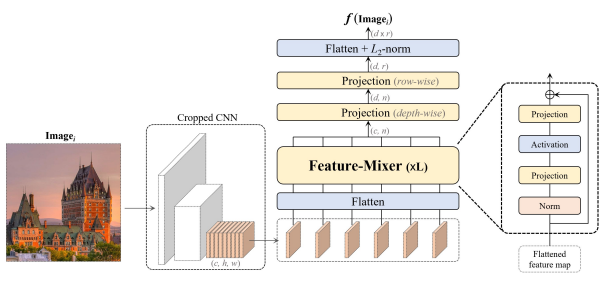
\includegraphics[scale=0.7]{pics/Proposal/mixvpr.png}
    \caption{Tổng quát quá trình xử lý ảnh của MixVPR \cite{alibey2023mixvpr}}
\end{figure}
Với ảnh đầu vào là $I$, mô hình CNN cơ sở sẽ trích xuất ra được tập Feature Map có dạng $F \in R^{c \cdot h \cdot w}$ từ những lớp trung gian.
$$
F = CNN(I)
$$
Ở những phương pháp trước như NetVLAD \cite{arandjelović2016netvlad} và PatchNetVLAD \cite{hausler2021patchnetvlad}, những lớp Feature Map thuộc $F$ sẽ được xem như là một mô tả tương ứng với một miền tiếp nhận cho một khu vực trong ảnh ban đầu. Ngược lại, MixVPR xem $F$ như một tập các bản đồ đặc trưng 2D có kích thước $h \cdot w$, miêu tả toàn ảnh. Mỗi giá trị trên bản đồ đặc trưng sẽ chứa thông tin mô tả một bộ phận của ảnh.
$$
F = \{X^{i}\}    i = \{1,...c\}
$$
với $X^{i}$ tương ứng với bản đồ kích hoạt thứ $i$ ở F. Ở cách biểu diễn này, mỗi Feature Map không chỉ đại diện cho một miền tiếp nhận trong ảnh mà sẽ chứa một loại thông tin đặc thù cho toàn bộ ảnh. $X^{i}$ sau đó sẽ được định dạng lại thành ma trận một chiều, có được $F \in R^{c \cdot n}$ với $n = h*w$.

Sau đó, dữ liệu sẽ được đưa qua khối Feature Mixer, gồm $L$ những lớp mạng MLP. Những lớp này sẽ nhận vào từng Feature Map $X^{i}$ một chiều và tích hợp thông tin về mối liên kết giữa các giá trị của $X^{i}$ lên chính nó thông qua cách sau:
$$
\begin{aligned}
    X^{i} & \leftarrow Norm(X^{i}) \\
    X^{i} & \leftarrow W_2(\sigma(W_1 X^{i}))
\end{aligned}
$$
với $W_1$ và $W_2$ là trọng số của hai lớp liên kết đầy đủ, cấu tạo nên MLP và $\sigma$ là hàm tạo sự phi tuyến tính cho quá trình xử lý(ReLU). Kỹ thuật nối tắt được sử dụng để nối đầu vào đã qua lớp chuẩn hóa với đầu ra nhằm giúp độ dốc trong quá trình huấn luyện có thể được truyền tải dễ hơn, cải thiện quá trình huấn luyện.

Mục đích của việc sử dụng Feature Mixer là để tận dụng khả năng tổng hợp thông tin từ dữ liệu của các lớp kết nối đầy đủ, thay vì học trên những đặc trưng cục bộ trên ảnh và sử dụng cơ chế tập trung. Ngoài ra, Feature Mixer cũng sẽ trả về kết quả có định dạng như cũ, thay vì có đầu ra giảm dần như những phương pháp tổng hợp dạng phân cấp(kim tự tháp) như trước đây, để mỗi nơ-ron đều có thể biết được thông tin của toàn bộ ảnh. Những lớp MLP trong khối Feature Mixer sẽ giúp tích hợp thông tin trên toàn bộ ảnh qua mỗi lần xử lý.

Mỗi khối Feature Mixer sau khi xử lý xong từng Feature Map trong tập $F \in R^{c \cdot n}$, sẽ ghép kết quả lại, tạo thành $Z \in R^{c \cdot n}$ với cùng kích thước trước khi được đưa vào khối Feature Mixer kế tiếp. Quá trình này có thể được miêu tả bằng công thức sau:
$$
Z = FM_L(FM_{L-1}(\dots FM_1(F)))
$$
Số chiều của $Z$ thường sẽ rất cao do có định dạng được giữ nguyên so với $F$. Để giúp giảm bớt số chiều của $Z$ lại sau khi qua khối Feature Mixer, hai lớp kết nối đầy đủ sẽ được sử dụng để tổng hợp giữa các kênh với nhau và sau đó là giữa các giá trị trong từng kênh. Tác vụ này thực hiện việc tổng hợp có chọn lọc nhằm điều khiển được kích thước của giá trị đầu ra.

Đầu tiên, dữ liệu sẽ được tổng hợp số kênh để biến định dạng của $Z$ từ $R^{c \cdot n}$ thành $R^{d \cdot n}$.
$$
Z' = W_d(Transpose(Z))
$$
với $W_d$ là trọng số của lớp kết nối đầy đủ đầu tiên.

Sau đó, giá trị trên từng kênh sẽ được tổng hợp lại, từ định dạng $R^{d \cdot n}$ thành $R^{d \cdot r}$.
$$
O = W_r(Transpose(Z'))
$$
với $W_r$ là trọng số của lớp kết nối đầy đủ thứ hai.

Kết quả $O$ cuối cùng, có định dạng là $R^{d \cdot r}$, sẽ được ép thành một chiều và chuẩn hóa theo L2 như những phương pháp VPR khác \cite{arandjelović2016netvlad,berton2022rethinking}. Cuối cùng, từ ảnh đầu vào $I$, mô hình sẽ trả về một đoạn mã hóa biểu diễn cho nội dung của ảnh. Đoạn mã hóa này sau đó có thể được dùng để so sánh với giá trị mã hóa của những hình khác nhằm tìm ảnh có độ tương đồng cao nhất với $I$.

\subsubsection*{Chi tiết hiện thực phương pháp}
\textbf{Cấu trúc:} Phương pháp tổng hợp sử dụng mô hình MixVPR sẽ được hiện thực trên framework PyTorch. Mô hình CNN cơ sở của MixVPR sẽ được cắt ở lớp áp cuối của mô hình ResNet. Dữ liệu đầu vào cho MixVPR sẽ là một tập các Feature Map có kích thước 20x20. Thao tác tổng hợp trong khối Feature Mixer sẽ sử dụng lớp Linear được cung cấp bởi PyTorch, theo sau đó là một lớp ReLU để tạo tính phi tuyến tính. Với lớp chuẩn hóa, LayerNorm của PyTorch sẽ được sử dụng. Cuối cùng, đầu ra cuối cùng của khối Feature Mixer sẽ được tổng hợp xuống một chiều không gian biểu diễn nhỏ hơn sử dụng hai lớp kết nối đầy đủ giữa các kênh với nhau và giữa các giá trị trong mỗi kênh, chứng minh là MixVPR là một cấu trúc chỉ sử dụng MLP. Số khối Feature Mixer được sử dụng sẽ luôn được giữ là $L=4$ trừ khi được quy định khác.

\textbf{Huấn luyện:} Mô hình MixVPR được đánh giá trong bài nghiên cứu sẽ sử dụng mô hình ResNet \cite{he2016deep} đã được huấn luyện trên tập ImageNet \cite{krizhevsky2012imagenet} làm cơ sở. Sau đó, mô hình sẽ được huấn luyện trên tập dữ liệu GSV-Cities \cite{Ali_bey_2022}. Đối hàm mất mát, hàm Multi-Similarity Loss \cite{wang2019multi} do hàm đã được chứng mình là hỗ trợ cho ra kết quả tốt với tác vụ VPR \cite{Ali_bey_2022}. Kích thước của một batch sẽ có $P$ = 120 địa điểm, mỗi địa điểm được miêu tả bởi 4 ảnh, tạo thành một batch có kích thước 480 ảnh. Phương tối ưu giảm độ dốc ngẫu nhiên - SGD sẽ được sử dụng với quán tính - momentum là 0.9 với giá trị suy giảm trọng số - weight decay là 0.001. Tốc độ học - learning rate sẽ được khởi tạo với giá trị 0.05 và sẽ được chia 3 sau mỗi 5 chu kỳ - epoch. Cuối cùng, mô hình sẽ được huấn luyện tối đa 30 chu kỳ - epoch với đầu vào là ảnh đã được chỉnh xuống kích thước 320x320.

\textbf{Đánh giá:} Để đánh giá, 5 tiêu chuẩn sẽ được sử dụng. Pitts250k-test \cite{6618963}, bao gồm 8k ảnh truy vấn và 83k ảnh tham khảo, được thu thập từ Google Street View và Pitts30k-test \cite{6618963} là một tập con của Pitts250k bao gồm 8k ảnh truy vấn và 8k ảnh tham khảo. Cả 2 tập dữ liệu Pittsburgh đều có những góc nhìn có độ lệch đáng kể. Tập dữ liệu SPED \cite{zaffar2021vpr} gồm 607 ảnh truy vấn và 607 ảnh tham khảo từ camera giám sát chứa những thay đổi lớn về độ sáng và về cảnh vật các mùa. MSLS \cite{warburg2020mapillary} được thu thập từ camera hành trình của xe hơi và cho rất nhiều góc nhìn đa dạng và sự thay đổi về độ sáng. Cuối cùng, Nordland \cite{zaffar2021vpr} là một tập dữ liệu chứa nhiều thử thách khi sử dụng ảnh thu thập được ở cả 4 mùa với camera được gắn trên tàu. Đơn vị đánh giá được sử dụng sẽ là recall@k, thể hiện tỷ lệ của truy xuất thành công trên tổng số lượng truy xuất. Một truy xuất hình sẽ được xem là thành công khi ảnh được truy xuất nằm trong vòng 25m xung quanh ảnh truy vấn.

\subsubsection*{Hiệu quả của phương pháp}
Khi so sánh trên những tập dữ liệu phản ánh môi trường thành thị, phương pháp sử dụng mô hình MixVPR đạt được kết quả vượt trội so với những mô hình SOTA đã được đề xuất trước nó, như CosPlace \cite{berton2022rethinking} và NetVLAD \cite{arandjelović2016netvlad}. Những tập dữ liệu được sử dụng đã bao quát hết những trường hợp có thể tác động xấu đến mô hình như góc nhìn đa dạng; thời tiết, mùa thay đổi; chênh lệch về độ sáng.

MixVPR cũng có khả năng giải quyết được những trường hợp mà những phương pháp trước gặp khó khăn như:
\begin{itemize}
    \item Kiến trúc lặp lại nhiều
    \item Góc nhìn thay đổi rõ rệt
    \item Đường chân trời
    \item Độ sáng chênh lệch lớn
    \item Gặp nhiều vật thể cản trở tầm nhìn
\end{itemize}
Tuy nhiên, mô hình vẫn sẽ gặp thất bại khi độ chênh lệch góc nhìn là quá lớn hoặc có quá nhiều vật cản.

\begin{figure}[H]
    \centering
    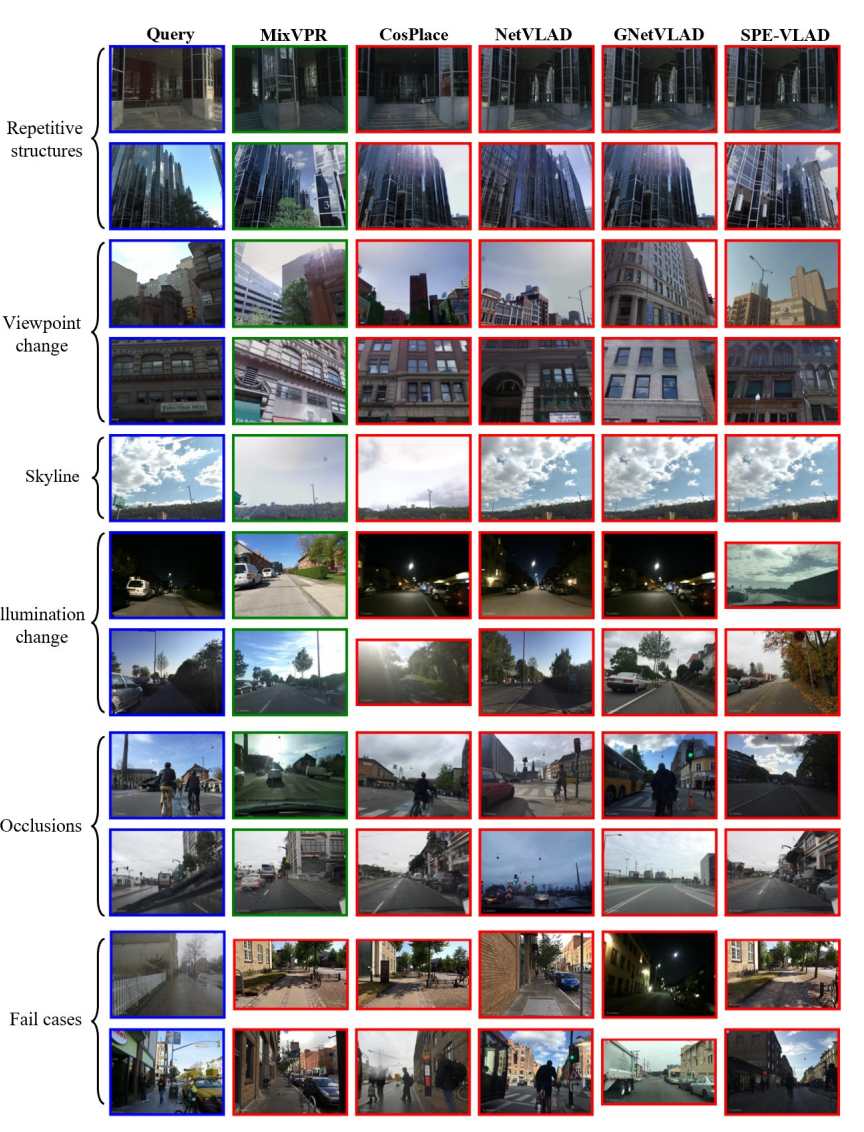
\includegraphics[scale=0.5]{pics/Proposal/fail.png}
    \caption{Kết quả của những trường hợp khó khi chạy trên MixVPR và các phương pháp khác \cite{alibey2023mixvpr}}
\end{figure}

Với sự ra đời của AnyLoc \cite{keetha2023anyloc}, bài toán VPR trong những môi trường đa dạng hơn như trong nhà, trong hang động, trên bầu trời, hoặc trên mặt biển đã có một SOTA mới. Điều này là nhờ việc AnyLoc sử dụng mạng cơ sở DINO, một mạng Vision Transformer được huấn luyện bằng cơ chế tự giám sát để sinh ra những đặc trưng có giá trị với mọi tác vụ. Tuy nhiên, khi xét đến môi trường thành thị thì MixVPR vẫn có cho ra kết quả chính xác hơn AnyLoc. Số liệu cụ thể sẽ được trình bày bên dưới.

\begin{figure}[H]
    \centering
    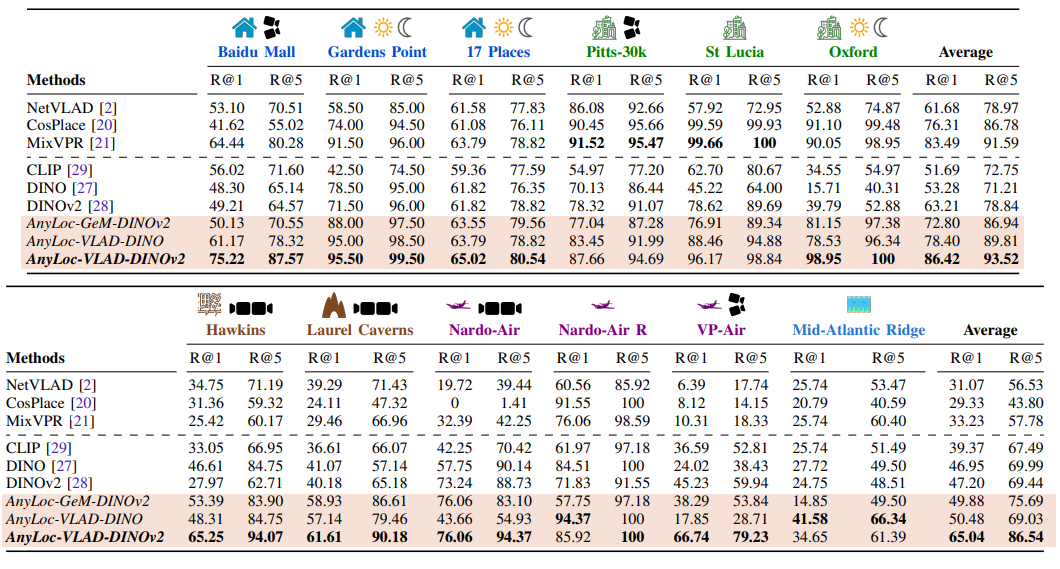
\includegraphics[scale=0.5]{pics/Proposal/anyloc.png}
    \caption{Kết quả của AnyLoc so sánh với những mô hình khác \cite{keetha2023anyloc}}
\end{figure}



\subsection{Mô hình tương quan 2D-2D của Map-free Relocalization \cite{arnold2022mapfree}}
\subsubsection*{Ý tưởng đằng sau mô hình}
Mô hình tương quan 2D-2D được đề xuất trong Map-free Relocalization thuộc nhóm những phương pháp sử dụng tìm kiếm cặp đặc trưng tương quan trong ảnh và xác định quy mô qua ước tính độ sâu. Phương pháp này sẽ giải quyết được điểm yếu của những phương pháp RPR là không nắm bắt được thông tin về hình học trong ảnh bằng cách sử dụng cách biểu diễn trung gian là ma trận thiết yếu. Dù kết quả của mô hình trong những môi trường có tập dữ liệu ảnh biểu diễn phân bố dày đặc là không quá vượt trội. Tuy nhiên, khi phân bố ảnh trong tập dữ liệu trở nên thưa hơn trong không gian đang xét thì phương pháp 2D-2D lại có kết quả vượt qua phương pháp 2D-3D và 3D-3D. 
\subsubsection*{Những bước xử lý của mô hình}

Với đầu vào là cặp ảnh $(I_A,I_B)$, những cặp đặc trưng tương quan giữa hai ảnh sẽ được xác định thành 2 tập là $(kpts_A, kpts_B)$ tương ứng với mỗi hình. Sau đó, ma trận thiết yếu giữa 2 ảnh sẽ được ước tính dựa vào giải thuật 5 điểm \cite{nister2004efficient} cùng với MAGSAC++ \cite{barath2020magsac++} dựa trên 2 tập điểm tương quan đã được xác định. Ma trận thiết yếu sau đó sẽ được phân giải thành ma trận thể hiện góc quay chênh lệch, $R \in SO(3)$ và vector đơn vị độ lệch về vị trí giữa hai ảnh, $\hat{t} \in R^{3}, \lvert \hat{t} \rvert = 1$.

Các cặp điểm tương quan giữa hai ảnh thỏa ma trận thiết yếu sẽ được chiếu lên không gian 3D qua độ sâu của ảnh. Với mỗi cặp điểm $(p_A,p_B)$, một tỷ lệ $s$ có thể được xác định bằng công thức:
$$
\begin{aligned}
    s=\underset{s^*}{\arg \min }\left\|R p_A+s^* \cdot \hat{t}-p_B\right\|_2 .
\end{aligned}
$$

\begin{figure}[H]
    \centering
    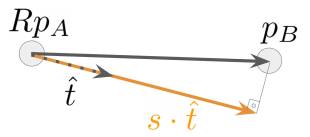
\includegraphics[scale=0.8]{pics/Proposal/reprojection.png}
    \caption[Minh họa cho việc xác định tỷ lệ $s$ bằng độ sâu ảnh]{Hình minh họa cho việc chiếu điểm $p_0$ qua vector góc quay $R$ và vector độ lệch đơn vị $\hat{t}$ cùng với tỷ lệ $s$ để tối thiểu khoảng cách \cite{arnold2022mapfree}}
\end{figure}


Mỗi cặp tương quan sẽ trả về một tỷ lệ $s$ cho vector đơn vị độ lệch. Vòng lặp RANSAC sẽ được sử dụng để loại bỏ những trường hợp ngoại lệ sinh ra từ việc ước lượng độ sâu sai lệch. Sau đó, giá trị $s$ có số cặp điểm hợp lệ lớn nhất sẽ được chọn để kiếm được vector độ lệch. Một cặp điểm sẽ được coi là hợp lệ nếu khoảng cách giữa hai điểm sau phép chiếu nhỏ hơn một giá trị nhất định. Trong bài nghiên cứu, giá trị 10cm được chọn.

\subsubsection*{Chi tiết hiện thực phương pháp}

\textbf{Cấu trúc:} Tác vụ tìm kiếm tương quan giữa hai ảnh sẽ có thể lựa chọn giữa phương pháp truyền thống như SIFT, hoặc những phương pháp theo hướng tiếp cận học sâu gần đây hơn như SuperPoint+SuperGlue \cite{sarlin2020superglue} và LoFTR \cite{sun2021loftr}. Tác vụ tính độ sâu đơn ảnh sẽ được phân thành hai trường hợp là bên trong nhà và ngoài trời. Với những tập dữ liệu trong nhà, mô hình DPT \cite{ranftl2021vision} được huấn luyện trên tập dữ liệu NYUv2 \cite{silberman2012indoor} PlaneRCNN \cite{liu2019planercnn} được huấn luyện trên tập dữ liệu ScanNet \cite{dai2017scannet}. Với trường hợp ngoài trời, mô hình DPT \cite{ranftl2021vision} được huấn luyện trên tập KITTI sẽ được sử dụng \cite{geiger2012we}.

\textbf{Đánh giá:} Để đánh giá hiệu quả của mô hình trong tác vụ định vị trực quan, một số tiêu chí cơ bản đã được đưa ra như độ lệch về góc quay, độ lệch về vị trí của máy ảnh, cũng như một sai số mới được đưa ra trong bài nghiên cứu, sai số phản chiếu của điểm 3D ảo - VCRE, được lấy cảm hứng từ sai số phản chiếu của những điểm tương ứng - DCRE \cite{wald2020beyond}. Cụ thể, với giá trị dự đoán $(R,t)$ và giá trị thực $(R_{gt},t_{gt})$, các sai số sẽ được xác định như sau:
\begin{itemize}
    \item Sai số về góc quay, $\measuredangle(R,R_{gt})$, sẽ được tính là độ chênh lệch giữa góc quay được dự đoán và góc quay thực tế.
    \item Sai số về độ lệch máy quay sẽ được tính là khoảng cách Euclidian giữa cặp vị trí $(c,c_{gt})$ được tính theo công thức $c=-R \intercal t$.
    \item Sai số phản chiếu của điểm 3D ảo sẽ được dùng để đánh giá độ lệch của những vật thể trong không gian thực tế ảo. Giá trị thực $(R_{gt},t_{gt})$ và giá trị dự đoán $(R,t)$ sẽ được dùng để chiếu những điểm 3D ảo, lên hệ tọa độ của camera truy vấn. Giá trị VCRE sẽ được xác định theo công thức
    $$
    \operatorname{VCRE}=\frac{1}{|\mathcal{V}|} \sum_{\mathbf{v} \in \mathcal{V}}\left\|\pi(\mathbf{v})-\pi\left(T T_{\mathrm{gt}}^{-1} \mathbf{v}\right)\right\|_2 \quad \text { với } T=[R \mid t]
    $$

    với $\pi$ là phép chiếu từ không gian camera lên ảnh, $\mathcal{V}$ là một tập các điểm 3D, đại diện cho những vật thể ảo. $\mathcal{V}$ là một lưới điểm 3D, (chiều cao là 4, chiều rộng là 7 và chiều sâu là 7), cách nhau 30cm và có độ dịch là 1.8m dọc theo trục của máy ảnh. Giá trị sai số của phép phản chiếu sẽ được so sánh với đường chéo của ảnh.
    \item Độ tin cậy của dự đoán cũng là một tiêu chí được đánh giá. Giá trị này cho phép mô hình có thể phát hiện và loại bỏ những dự đoán không đáng tin cậy. Giá trị này sẽ được xác định bằng số lượng cặp điểm tương quan thỏa ma trận thiết yếu được chọn trên tổng số cặp điểm tương quan xác định bởi mô hình ghép đặc trưng. Với một ngưỡng tin cậy nhất định, tỷ lệ dự đoán đáng tin cậy - ratio of confident estimate, sẽ được xác định là tỷ lệ của những ảnh truy vấn có độ tin cậy vượt qua ngưỡng.
    \item Độ chính xác của mô hình sẽ là tỷ lệ của những ảnh đáng tin cậy có sai lệch giữa giá trị dự đoán và giá trị thực dưới một ngưỡng nhất định (độ lệch vị trí và góc quay) hoặc có sai số phản chiếu chấp nhận được trên tổng số ảnh.
\end{itemize}

Tập dữ liệu 7Scenes \cite{6619221} sẽ được sử dụng để xác định hiệu quả của mô hình tiêu chuẩn của Mapfree sẽ có hiệu quả như thế nào so với những phương pháp SOTA tại thời điểm đó, với số lượng ảnh tham khảo là rất nhiều. Ảnh hưởng của việc giảm số lượng ảnh tham khảo lên khả năng hoạt động của các mô hình cũng sẽ được ghi nhận lại. Tập dữ liệu Niantic được đề xuất trong cùng bài nghiên cứu cũng sẽ được sử dụng để đánh giá, nhằm xác định hiệu quả của các mô hình trong trường hợp chỉ có một ảnh tham khảo.

\subsubsection*{Hiệu quả của phương pháp}

\textbf{Tập dữ liệu 7Scenes \cite{6619221}}

\begin{figure}[H]
    \centering
    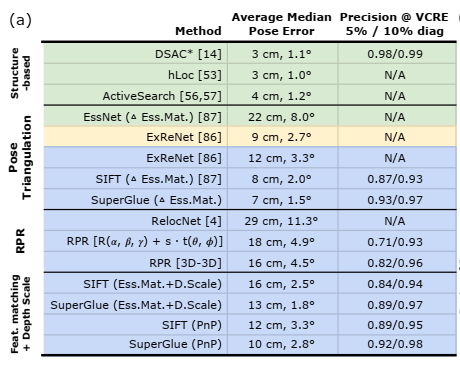
\includegraphics[scale=0.8]{pics/Proposal/all_7scene.png}
    \caption[Bảng so sánh hiệu quả của các mô hình trên tập 7Scenes]{Hiệu quả của những mô hình khi có đầy đủ ảnh tham khảo trên tập 7Scenes. Những phương pháp \textcolor{green}{xanh lá} sẽ phụ thuộc vào tập dữ liệu, phương pháp \textcolor{yellow}{vàng} được huấn luyện trên SUNCG \cite{song2017semantic} và \textcolor{blue}{xanh dương} trên tập ScanNet \cite{dai2017scannet}}
\end{figure}

Khi xét trên tập dữ liệu 7Scenes với tất cả các ảnh tham khảo, những phương pháp sử dụng biểu diễn 3D như DSAC* \cite{brachmann2021visual}, hLoc \cite{sarlin2019coarse}, ActiveSearch \cite{sattler2016efficient} có kết quả tốt nhất, tuy nhiên lại phụ thuộc vào quá trình tái tạo lại cấu trúc. Những phương pháp sử dụng phép đạc tam giác, sử dụng 5 ảnh tham khảo có kết quả cạnh tranh so với những phương pháp sử dụng biểu diễn 3D, được ký hiệu bằng $\triangle$. 

Để thực hiện bài toán định vị không cần biểu diễn, chỉ một ảnh tham khảo sẽ được sử dụng cho một truy vấn cho những phương pháp trong tập \textit{hồi quy vị trí tương đối} và \textit{ghép cặp đặc trưng + độ sâu ảnh}. Cả hai lớp phương pháp đều có kết quả bị xuống cấp, với phương pháp ghép cặp + độ sâu tốt hơn những phương pháp hồi quy tương đối. Tuy nhiên, các phương pháp thuộc các lớp vẫn có kết quả cạnh tranh, có thể được phần nào giải thích bởi việc truy xuất ảnh tốt và sự phân bố dày đặc của tập dữ liệu.

\begin{figure}[H]
    \centering
    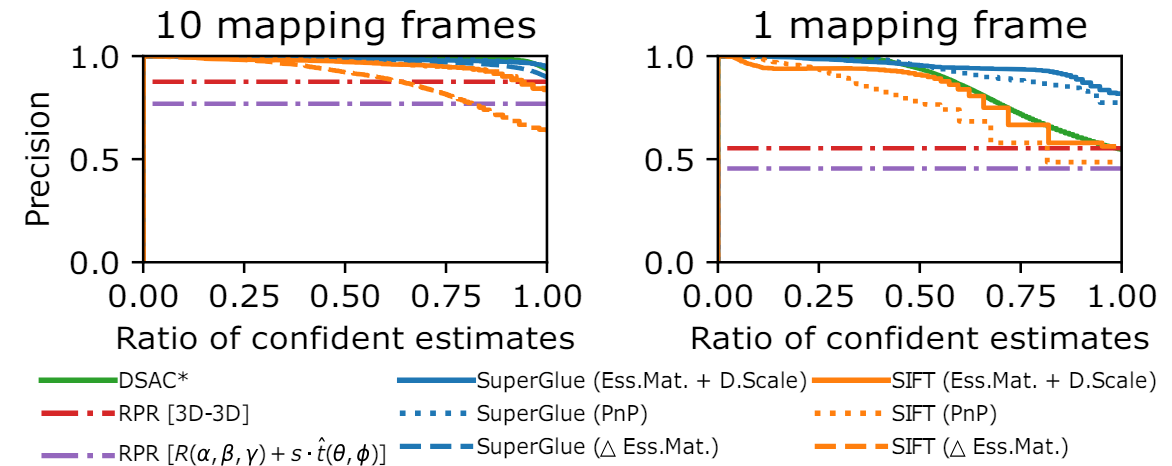
\includegraphics[scale=0.8]{pics/Proposal/partial_7scene.png}
    \caption[Hiệu quả của các mô hình khi giới hạn ảnh tham khảo]{Hiệu quả của những mô hình khi tập 7Scenes chỉ có 10/1 ảnh tham khảo, đánh giá về độ chính xác và về số ảnh có sai số phản chiếu dưới ngưỡng.}
\end{figure}

Để có thể phản ánh một môi trường thực, nơi mà ảnh tham khảo truy xuất được cách xa đáng kể so với ảnh truy vấn, $K$ ảnh tham khảo mang nhiều thông tin nhất sẽ được chọn làm đại diện qua giải thuật gom cụm K-means.

Với việc so sánh độ chính xác ở hai kịch bản, ngưỡng chấp nhận về độ chính xác sẽ là $VCRE<10\%$ của đường chéo ảnh(80px). Khi ngưỡng tin cậy được hạ thấp, điều này làm cho tỷ lệ dự đoán đáng tin cậy tăng lên. Điều này làm độ chính xác giảm dần, do chứa những trường hợp có độ tin cậy không đủ cao. Trong trường hợp này, những mô hình 2D-2D, đặc biệt là mô hình sử dụng SuperGlue, có kết quả tốt hơn so với những mô hình còn lại, đặc biệt trong khoảng $0.5~1.0$. Ngoài ra, mô hình 2D-2D có thể tính ra vị trí và góc quay của hơn 50\% ảnh với VCRE < 40px.

Mô hình DSAC* vẫn có kết quả tốt nhất trong các mô hình. Tuy nhiên, phương pháp này lại phụ thuộc vào tập dữ liệu. Trong khi đó, những mô hình khác được huấn luyện trên tập ScanNet vẫn có kết quả tốt trên tập 7Scenes. Phương pháp sử dụng phép đạc tam giác cũng có kết quả cạnh tranh, tuy nhiên lại không thể hoạt động chỉ với một ảnh tham khảo. Những phương pháp ghép cặp + độ sâu có khả năng khái quát hóa tốt hơn những phương pháp RPR, như có thể thấy ở hiệu quả thấp hơn của những phương pháp hồi quy tương đối.

\textbf{Tập dữ liệu Niantic \cite{arnold2022mapfree}}

\begin{figure}[H]
    \centering
    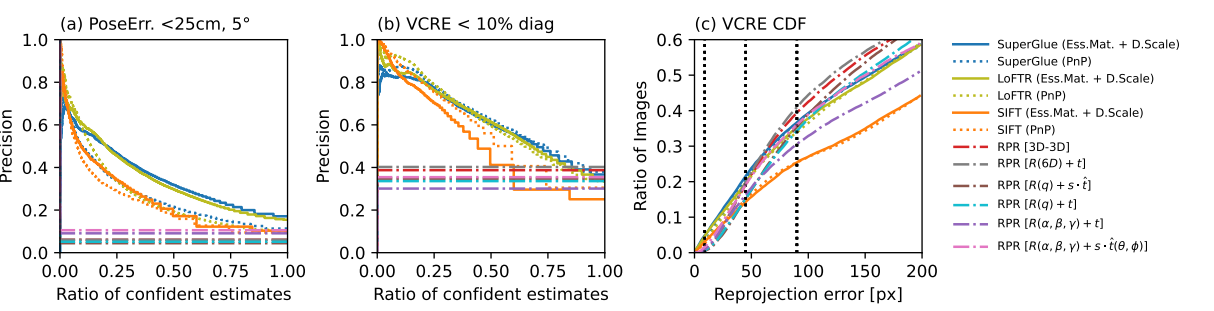
\includegraphics[scale=0.4]{pics/Proposal/all_niantic.png}
    \caption{Hiệu quả của các mô hình trên tập dữ liệu Niantic, xác định theo độ chính xác và số ảnh có sai số phản chiếu dưới ngưỡng}
\end{figure}

Qua kết quả thu được, tập dữ liệu Niantic có độ khó cao hơn đáng kể so với tập dữ liệu 7Scenes với mọi phương pháp. Điều này có thể thấy được rõ ràng từ kết quả của các mô hình. Trong tập dữ liệu Mapfree, những phương pháp 2D-2D tiếp tục có kết quả tốt. Tuy nhiên, ở những ngưỡng VCRE rộng hơn, những phương pháp RPR lại có kết quả tốt hơn. Điều này có thể giải thích được qua việc khi số cặp đặc trưng tương quan là không đủ chất lượng, độ lệch đơn vị vị trí được sinh ra có thể có sai số rất lớn so với thực tế. Vậy nên, những phương pháp RPR sẽ cho ra kết quả tốt khi ngưỡng chính xác rộng, nhưng lại có kết quả không tốt khi cần độ chính xác cao. Ngoài ra, những phương pháp RPR cũng không thể cung cấp độ tin cậy cho dự đoán của mô hình, hạn chế việc loại bỏ những dự đoán có khả năng sai cao.

\section{Mô hình đề xuất}
\subsection{Tổng quan}
Gọi $I$ là ảnh mà người dùng chụp từ máy ảnh và sẽ được dùng làm ảnh truy vấn cho mô hình đề xuất của nhóm. Trước hết, mô hình sẽ nhận $I$ và truyền làm đầu vào cho MixVPR. Từ ảnh đầu vào $I$, sau khi qua các giai đoạn xử lý, MixVPR sẽ trả về một đoạn mã hóa biểu diễn cho nội dung của ảnh. Với đoạn mã hóa này, mô hình tiến hành so sánh với giá trị mã hóa của các ảnh trong cơ sở dữ liệu và tìm ra ảnh có sự tương đồng cao nhất với ảnh nhận vào $I$ gọi là $I_0$.

Bước tiếp theo, mô hình tiếp tục truyền cả ảnh nhận vào $I$ và ảnh được truy xuất $I_0$ cho mô hình tương quan 2D - 2D của Map-free Relocalization \cite{arnold2022mapfree}. Với đầu vào là cặp ảnh $(I, I_0)$, những cặp đặc trưng tương quan giữa hai ảnh sẽ được xác định tương ứng với mỗi hình. Sau đó, ma trận thiết yếu $E$ giữa 2 ảnh sẽ được ước tính. Ma trận thiết yếu sau đó sẽ được phân giải thành ma trận thể hiện góc quay chênh lệch $R$ và một véc-tơ đơn vị độ dịch vị trí $\hat{t}$. Từ các cặp đặc trưng và độ sâu của ảnh, mô hình tiến hành một bước chiếu 3D để tính toán giá trị tỷ lệ $s$ của véc-tơ độ dịch vị trí. Cuối cùng, vị trí thực của máy ảnh sẽ được xác định bằng vị trí thực của ảnh tham khảo và độ lệch giữa ảnh tham khảo và ảnh truy vấn $(R,s*\hat{t})$.

\subsection{Dữ liệu đầu vào và đầu ra}
Mô hình sẽ nhận vào ảnh $I$, có định dạng là một ảnh có 3 kênh màu đỏ, xanh lá và xanh dương. Sau đó, ảnh $I$ sẽ được tiền xử lý, gồm các bước đưa về định dạng RGB, kích thước 320x320 và chuẩn hóa các điểm ảnh trên hình, trước khi được đưa vào mô hình chính.

Định dạng đầu ra của mô hình sẽ gồm hai tập vector $R$ và $t$, lần lượt thể hiện góc quay và vị trí chụp ảnh trong không gian 3D. Cụ thể, hai vector sẽ có dạng:
\begin{itemize}
    \item \textbf{Vector góc quay $R$} sẽ có định dạng của một Quaternion, gồm 4 số là $(q_w,q_x,q_y,q_z)$. Quaternion có thể được dùng để biểu diễn góc quay trong không gian 3D và có thể dùng để thay thế ma trận xoay 3x3, nhằm có thể thể hiện và kết hợp các phép quay một cách dễ dàng hơn. Công thức biểu diễn một góc quay là 
    $$
    q=q_w + i*q_x + j*q_y + k*q_z
    $$
    với $q_w, q_x, q_y, q_z$ là các số thực với $i,j,k$ là những vector đơn vị trực giao lẫn nhau. Quaternion có thể được biến đổi theo dạng trục quay và góc quay, có thể được biểu diễn bởi hai thành phần là vector đơn vị biểu diễn trục của góc quay, $(\hat{x},\hat{y},\hat{z})$ và độ quay quanh trục, $\theta$. 
    \begin{figure}[H]
        \centering
        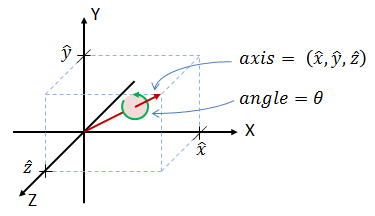
\includegraphics[scale=1]{pics/Proposal/axis-angle.png}
        \caption{Minh họa cách biểu diễn trục quay và góc quay \cite{quaternion}}
    \end{figure}
    Quaternion có thể được ước tính từ cách biểu diễn trục quay và góc quay theo công thức
    $$
    \begin{aligned}
        & q_w=\cos \left(\frac{\theta}{2}\right) \\
        & q_x=\hat{x} \sin \left(\frac{\theta}{2}\right) \\
        & q_y=\hat{y} \sin \left(\frac{\theta}{2}\right) \\
        & q_z=\hat{z} \sin \left(\frac{\theta}{2}\right)
    \end{aligned}
    $$
    Từ công thức, tập các giá trị $q_w, q_x, q_y, q_z$ có độ lớn là 1, dẫn đến tập các giá trị này sẽ có 3 độ tự do, 3DoF.
    \item \textbf{Vector vị trí $t$} sẽ có 3 giá trị là $t_x,t_y,t_z$ lần lượt thể hiện các giá trị kinh độ, vĩ độ và độ cao của vị trí chụp ảnh trong không gian thực tế. Vector thể hiện vị trí có cách biểu diễn đơn giản và dễ hiểu hơn so với góc quay. Ngoài ra, do biểu diễn không gian 3 chiều thực tế nên vector thể hiện vị trí sẽ có 3 độ tự do.
\end{itemize}

\subsection{Kiến trúc của mô hình đề xuất}
\begin{figure}[H]
    \centering
    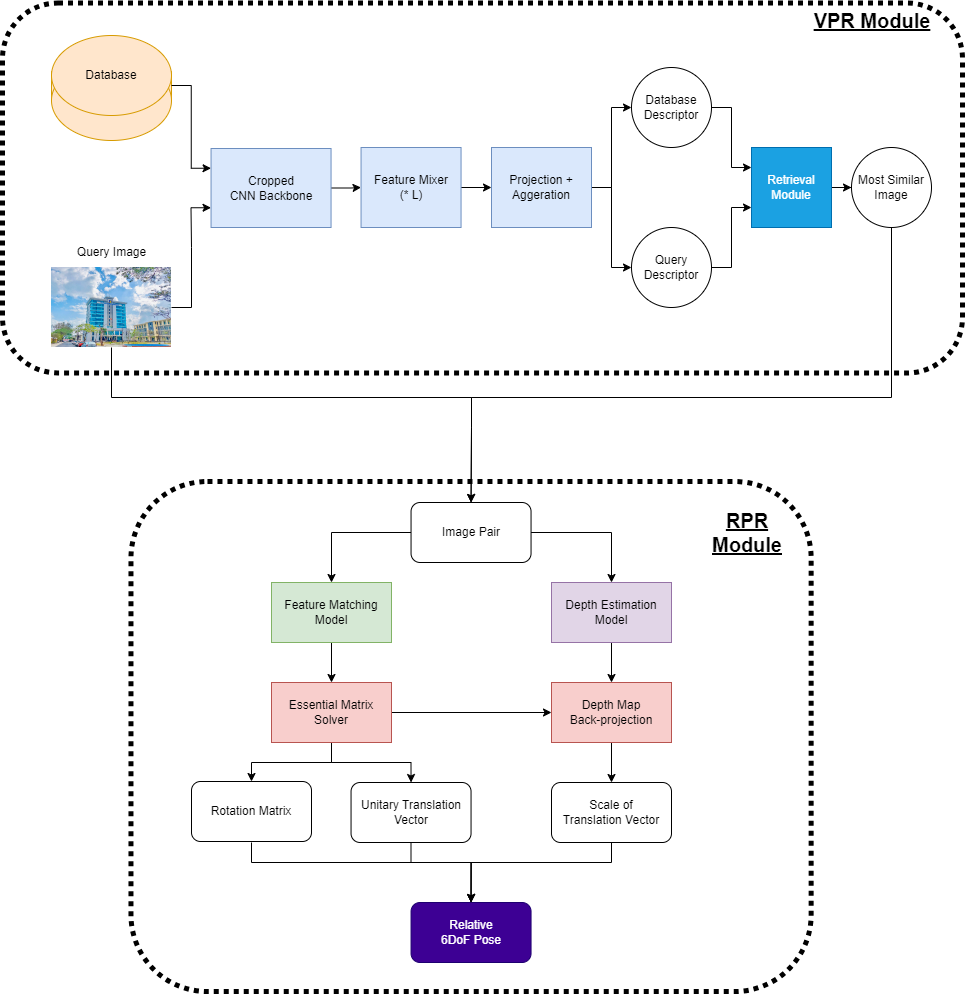
\includegraphics[scale=0.4]{pics/Proposal/models.png}
    \caption{Minh họa mô hình đề xuất}
\end{figure}

\subsubsection{Bộ phận nhận diện địa điểm trực quan - VPR}
\paragraph*{Mô hình cơ sở CNN}

Khi ảnh truy vấn $I$ được đưa vào, mô hình cơ sở CNN sẽ được sử dụng để trích xuất ra những chi tiết mang thông tin cần thiết. Mô hình cơ sở sẽ được huấn luyện trên những tập dữ liệu hình ảnh đa dạng, nhằm có thể phát hiện ra những chi tiết quan trọng cho các tác vụ liên quan đến thị giác máy tính. Trong kiến trúc đề xuất, mô hình cơ sở sẽ được cắt ở giữa, nhằm thu được tập những bản đồ đặc trưng $F$ có định dạng $c \cdot h \cdot w$. Mỗi giá trị trên bản đồ đặc trưng $h \cdot w$ sẽ chứa thông tin mô tả của hình ảnh tại vùng đó. Những bản đồ đặc trưng là một cách biểu diễn hình ảnh nhỏ, nhẹ và thống nhất hơn trong điều kiện thay đổi về ánh sáng và góc nhìn, thay cho việc lưu trữ từng điểm ảnh. Mỗi bản đồ đặc trưng thuộc tập $F$ sau đó sẽ được làm phẳng thành 1D và đưa vào làm đầu vào cho những lớp tiếp theo.

\begin{figure}[H]
    \centering
    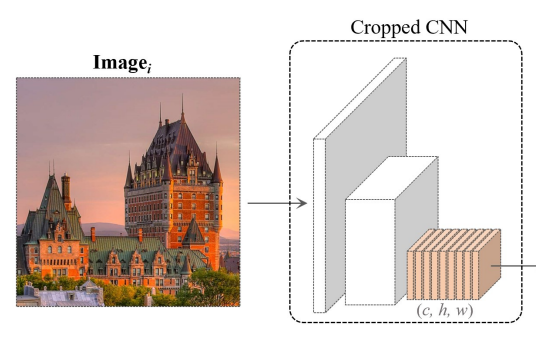
\includegraphics[scale=0.75]{pics/Proposal/cropped-cnn.png}
    \caption{Mô hình cơ sở xử lý ảnh để tạo ra tập các bản đồ đặc trưng \cite{alibey2023mixvpr}}
\end{figure}

\paragraph*{Những lớp Feature Mixer}

Dữ liệu đầu vào sẽ là một tập các bản đồ đặc trưng 1D, có cấu tạo $c \cdot h*w$. Mỗi lớp Feature Mixer sẽ được cấu tạo từ 4 lớp, theo thứ tự là lớp chuẩn hóa đầu vào $NormLayer$, lớp kết nối đầy đủ $W_1$, lớp kích hoạt để thêm sự phi tuyến tính vào kết quả $\sigma$ và lớp kết nối đầy đủ thứ hai $W_2$. Đầu ra sẽ là kết quả của lớp kết nối đầy đủ thứ hai được nối tắt với dữ liệu đầu vào, có định dạng $h*w$. Trừ khi được nêu khác, $L=4$ lớp Feature Mixer sẽ được sử dụng trong mô hình. Lớp Feature Mixer sẽ được áp dụng cho mỗi bản đồ đặc trưng 1D và giữ nguyên cấu tạo của dữ liệu đầu vào. Vậy nên, kết quả đầu ra vẫn sẽ là bản đồ đặc trưng có dạng $h*w$, được ghép lại thành ma trận có dạng $c \cdot h*w$.

$$
\begin{aligned}
    X^{i} & \leftarrow Norm(X^{i}) \\
    X^{i} & \leftarrow W_2(\sigma(W_1 X^{i}))
\end{aligned}
$$

$$
Z = FM_L(FM_{L-1}(\dots FM_1(F)))
$$

Lớp Feature Mixer sẽ giúp tích hợp thông tin toàn cục của ảnh, phân bố trên toàn bản đồ đặc trưng, vào các giá trị trên bản đồ đặc trưng. Vì vậy nên, định dạng của đầu vào và đầu ra của các lớp kết nối đầy đủ $W_1$ và $W_2$ sẽ giống nhau. Ngoài ra, trọng số của các lớp này sẽ được chia sẻ giữa các bản đồ đặc trưng nhằm tối ưu quá trình huấn luyện.

\begin{figure}[H]
    \centering
    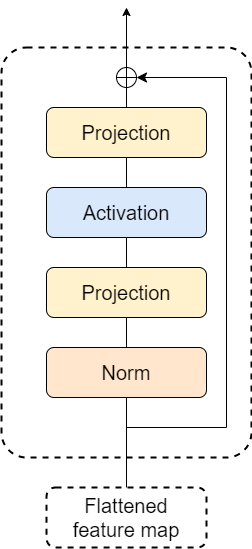
\includegraphics[scale=0.75]{pics/Proposal/mixer.png}
    \caption{Cấu tạo của một lớp Feature Mixer \cite{alibey2023mixvpr}}
\end{figure}

\paragraph*{Lớp tổng hợp}

Sau khi chạy qua $L$ lớp Feature Mixer và ghép lại với nhau, kết quả sẽ ở dạng $c \cdot h*w$. Do thông tin của kết quả thường sẽ được miêu tả trong không gian có số chiều lớn, lớp tổng hợp sẽ được sử dụng để thu nhỏ lại kết quả. Các lớp tổng hợp được chạy lần lượt là tổng hợp giữa các bản đồ đặc trưng $W_d$, và tổng hợp các giá trị trong mỗi bản đồ đặc trưng $W_r$. Lớp tổng hợp giữa các bản đồ đặc trưng sẽ thu gọn ma trận đặc trưng từ $c \cdot h*w$ thành $d \cdot h*w$. Sau đó, lớp tổng hợp các giá trị trên bản đồ đặc trưng sẽ trả về kết quả là $d \cdot r$.

$$
\begin{aligned}
Z' &= W_d(Transpose(Z))
O &= W_r(Transpose(Z'))
\end{aligned}
$$

Cuối cùng, kết quả sẽ được làm phẳng thành 1D và lấy chuẩn hóa theo L2 để tạo thành kết quả cuối cùng là giá trị mã hóa biểu diễn cho ảnh. Vector kết quả sẽ có dạng $d*r$.

\begin{figure}[H]
    \centering
    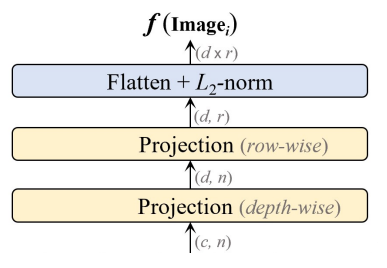
\includegraphics[scale=0.75]{pics/Proposal/proj-agg.png}
    \caption{Quá trình tổng hợp của mô hình \cite{alibey2023mixvpr}}
\end{figure}

\paragraph*{Bộ phận truy vấn ảnh tương đồng}

Sau khi đã có được giá trị mã hóa biễu diễn cho ảnh truy vấn, mô hình sẽ tiến hành tìm kiếm trên tập dữ liệu ảnh miêu tả khu vực đang xét. Cơ chế tìm kiếm được sử dụng sẽ là tìm kiếm toàn diện, xét giá trị biểu diễn của từng ảnh. $k$ ảnh có độ tương đồng cao nhất với ảnh truy vấn sẽ được chọn để tạo thành các cặp ảnh là đầu ra của bước này.

\begin{figure}[H]
    \centering
    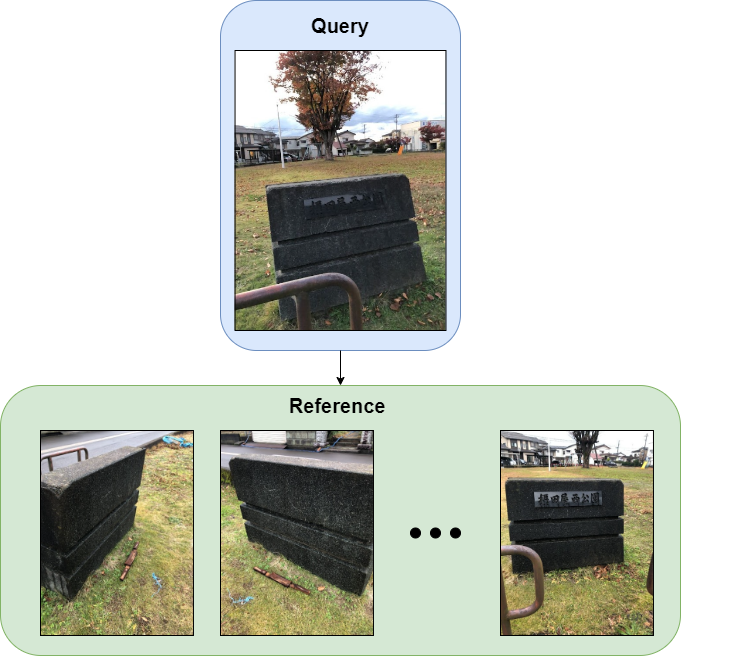
\includegraphics[scale=0.5]{pics/Proposal/query.png}
    \caption[Kết quả của module VPR]{Ảnh truy xuất được từ ảnh truy vấn $I$ ban đầu, từ tập dữ liệu Niantic \cite{arnold2022mapfree}}
\end{figure}

\paragraph*{Kết quả}

Qua quá trình mô phỏng lại bài toán nhận diện địa điểm trực quan, mô hình sẽ thuc được $k$ cặp ảnh có độ tương đồng cao, với một trong số đó là ảnh truy vấn ban đầu. Từng cặp ảnh trong $k$ cặp này sẽ được đưa vào bộ phận hồi quy vị trí tương đối tiếp theo.

\subsubsection{Bộ phận hồi quy vị trí tương đối - RPR}
\paragraph*{Mô hình xác định cặp đặc trưng + ước tính độ sâu của ảnh}

Với dữ liệu đầu vào là cặp ảnh gồm ảnh truy vấn và ảnh tham khảo $(I,I_0)$, tại bước này, những cặp đặc trưng tương quan sẽ được xác định và vị trí của chúng sẽ được lưu lại trong 2 tập là $(kpts_0,ktps_1)$ và bản đồ chứa thông tin thông tin về độ sâu của mỗi ảnh cũng sẽ được sinh ra. Mô hình ghép đặc trưng được sử dụng sẽ là SuperPoint+SuperGlue \cite{sarlin2020superglue} đã trải qua quá trình huấn luyện Mô hình dự đoán độ sâu được sử dụng sẽ là mô hình DPT \cite{ranftl2021vision} được huấn luyện trên tập KITTI do phạm vi được sử dụng của mô hình sẽ là ở ngoài trời, trong khu vực thành thị \cite{arnold2022mapfree}. Dữ liệu trả về của 2 mô hình này sẽ là hai tập chứa vị trí của các điểm đặc trưng tương ứng và bản đồ độ sâu ước tính của mỗi hình.

\begin{figure}[H]
    \centering
    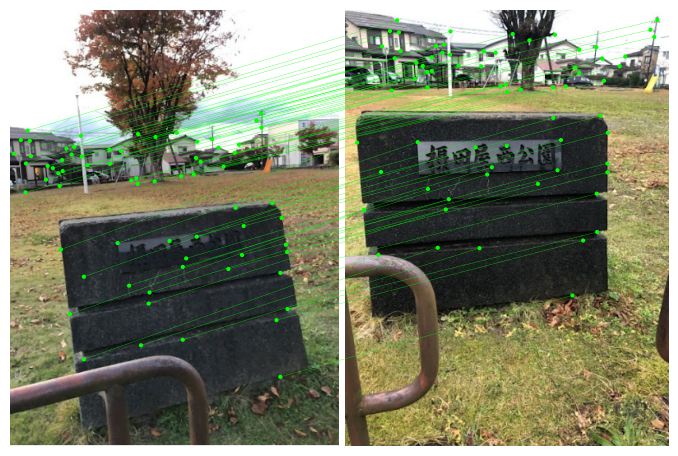
\includegraphics[scale=0.7]{pics/Proposal/matching.png}
    \caption{Kết quả của quá trình xác định và ghép đặc trưng}
\end{figure}

\begin{figure}[H]
    \centering
    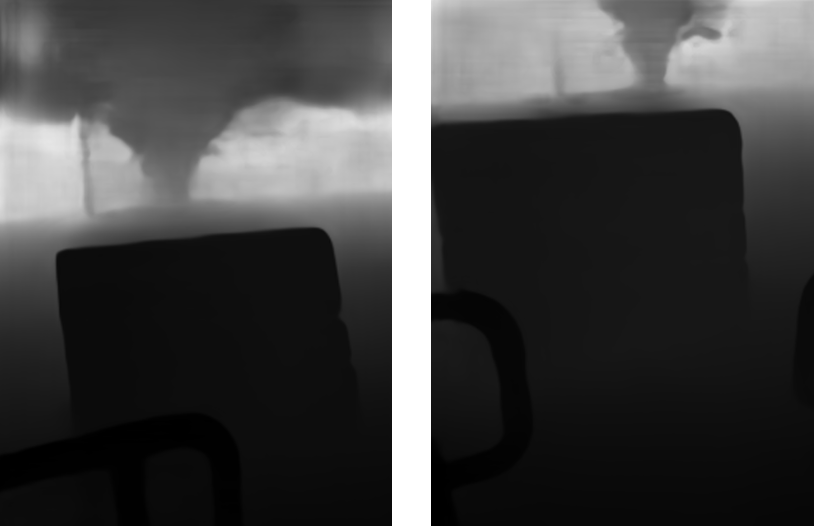
\includegraphics[scale=0.6]{pics/Proposal/depth.png}
    \caption{Kết quả của quá trình ước tính độ sâu ảnh}
\end{figure}

\paragraph*{Bộ phận xác định ma trận thiết yếu}

Dựa vào những cặp đặc trưng tương quan đã được xác định trong các tập $(kpts_0, kpts_1)$ và ma trận thông số của camera, ma trận thiết yếu $M$ sẽ được xác định qua giải thuật 5 điểm và vòng lặp MAGSAC++. Ma trận thông số của camera sẽ chứa các thông tin về tiêu cự của máy ảnh $f_x,f_y$ và tọa độ điểm chính của máy ảnh $c_x,c_y$, được sắp xếp thành ma trận như sau:
$$
c = \begin{bmatrix} f_x & 0 & c_x \\ 0 & f_y & c_y \\ 0 & 0 & 1 \end{bmatrix}
$$ 
Qua ma trận thiết yếu $M$, ma trận thể hiện độ lệch góc quay $R$ và vector thể hiện đơn vị độ lệch vị trí $\hat{t}$ giữa hai camera sẽ được xác định. Tập những cặp điểm tương quan thỏa ma trận thiết yếu $M$ cũng sẽ được trả về, được sử dụng để đánh giá độ đang tin cậy của dự đoán.



\paragraph*{Bộ phận chiếu cặp điểm tương quan lên không gian 3D}

Những cặp điểm tương quan thỏa ma trận $M$ sau đó sẽ được chiếu lên không gian 3D qua bản đồ độ sâu ảnh đã được sinh ra ở mỗi ảnh. Với mỗi cặp điểm $p_A,p_B$ đã được chiếu lên không gian 3D, mô hình sẽ tìm được một giá trị tỷ lệ $s$ cho $\hat{t}$ để làm giảm thiểu độ lệch của điểm $p_A$ khi được chiếu lên hệ tọa độ của camera thứ hai và điểm $p_B$. Giá trị $s$ tương ứng với mỗi cặp điểm $(p_A,p_B)$ có thể được xác định qua công thức:

$$
\begin{aligned}
    s=\underset{s^*}{\arg \min }\left\|R p_A+s^* \cdot \hat{t}-p_B\right\|_2 .
\end{aligned}
$$

Cuối cùng, tỷ lệ $s$ với số cặp điểm hợp lệ cao nhất sẽ được chọn làm kết quả cuối cùng. Một cặp điểm sẽ được xem như hợp lệ khi khoảng cách sai lệch giữa hai điểm 3D sau khi chiếu nhỏ hơn một ngưỡng nhất định, ở đây được xác định là 10cm. Vòng lặp RANSAC sẽ được sử dụng để bỏ những trường hợp ngoại lệ.

Sau khi chạy qua những bước trên, mô hình sẽ thu về được các giá trị thể hiện độ lệch giữa vị trí và góc quay của cặp ảnh truy vấn và tham khảo dưới dạng ma trận độ lệch góc quay $R$ và vector độ lệch vị trí $s*\hat{t}$. Ma trận độ lệch góc quay $R$ sau đó sẽ được phân giải thành một Quaternion, được biểu diễn dưới dạng một tập 4 số là $(q^{\Delta}_w,q^{\Delta}_x,q^{\Delta}_y,q^{\Delta}_z)$ thể hiện góc quay trong không gian. Vector độ lệch vị trí sẽ có dạng bộ 3 số là $(t^{\Delta}_x,t^{\Delta}_y,t^{\Delta}_z)$. 

\paragraph*{Bộ phận chuyển đổi sang vị trí tuyệt đối}

Từ hai tập 4 số này, mô hình đã biểu diễn được góc quay và vị trí tương đối giữa hai ảnh $(q^{\Delta},t^{\Delta})$. Khi biết được tọa độ chính xác của ảnh tham khảo $(q^{ref},t^{ref})$, mô hình sẽ tính ra được tọa độ và góc quay chính xác của ảnh truy vấn và đưa ra kết quả cuối cùng là hai tập $(q^{abs},t^{abs})$

Để xác định được góc quay chính xác của ảnh truy vấn, mô hình biến đổi góc quay của ảnh tham khảo với độ lệch góc quay đã xác định được giữa hai ảnh theo công thức:

$$
\begin{aligned}
    q^{abs} &= q^{\Delta} * q^{ref} \\
    (q^{abs}_w,q^{abs}_x,q^{abs}_y,q^{abs}_z) &= (q^{\Delta}_w,q^{\Delta}_x,q^{\Delta}_y,q^{\Delta}_z) * (q^{ref}_w,q^{ref}_x,q^{ref}_y,q^{ref}_z) \\ \\
    q^{abs}_w &=\left(q^{\Delta}_w q^{ref}_w-q^{\Delta}_x q^{ref}_x-q^{\Delta}_y q^{ref}_y-q^{\Delta}_z q^{ref}_z\right) \\
    q^{abs}_x &=\left(q^{\Delta}_w q^{ref}_x+q^{\Delta}_x q^{ref}_w-q^{\Delta}_y q^{ref}_z+q^{\Delta}_z q^{ref}_y\right) \\
    q^{abs}_y &=\left(q^{\Delta}_w q^{ref}_y+q^{\Delta}_x q^{ref}_z+q^{\Delta}_y q^{ref}_w-q^{\Delta}_z q^{ref}_x\right) \\
    q^{abs}_z &=\left(q^{\Delta}_w q^{ref}_z-q^{\Delta}_x q^{ref}_y+q^{\Delta}_y q^{ref}_x+q^{\Delta}_z q^{ref}_w\right)
\end{aligned}
$$

Để xác định được vị trí chính xác của ảnh truy vấn trong không gian thực, vị trí kinh độ, vĩ độ và độ cao của ảnh chụp có thể được xác định qua công thức:

$$
\begin{aligned}
    t^{abs} &= t^{\Delta} + t^{ref} \\
    (t^{abs}_x,t^{abs}_y,t^{abs}_z) &= (t^{\Delta}_x,t^{\Delta}_y,t^{\Delta}_z) + (t^{ref}_x,t^{ref}_y,t^{ref}_z) \\ \\
    t^{abs}_x &= t^{\Delta}_x + t^{ref}_x \\
    t^{abs}_y &= t^{\Delta}_y + t^{ref}_y \\
    t^{abs}_z &= t^{\Delta}_z + t^{ref}_z \\
\end{aligned}
$$

\paragraph*{Kết quả}

Kết quả đầu ra của bộ phận này sẽ là hai tập số $(q^{abs},t^{abs})$ thể hiện vị trí và góc quay của ảnh truy vấn trong không gian 3D.

Sau khi đã có được vị trí của ảnh $I$ khi so với tập $k$ ảnh tham khảo có độ tương đồng cao nhất, mô hình sẽ chọn ra kết quả cuối cùng dựa vào độ đáng tin cậy được xác định ở \textbf{Bộ phận xác định ma trận thiết yếu}. Dự đoán nào có số cặp điểm tương quan thỏa ma trận thiết yếu $M$ được chọn cao nhất sẽ được dùng làm dự đoán cuối cùng của mô hình.